%!TEX root = ../../../../report.tex
\subsection{Mechanical limits} % (fold)
\label{sub:mechanical_limits}
The design includes mechanical limits that are used for two reasons:
\begin{enumerate}
  \item \textbf{Calibration}: used as starting points for the relative encoders.
  \item \textbf{Security}: the mechanical limits do not allow the movement further them, which restrict the movement to a predictible behavior protecting then other parts of the robot.
\end{enumerate}

The figure \ref{fig:joint_limits_hip} shows how the mechanical limits of the hip (both left and right) are implemented in the upper part, spreading an angle of 90 + 60 = 150 degrees.
The figure \ref{fig:joint_limits_ankle_upper} shows the upper part of the ankle and how the movement of the foot can be of 60 + 50 = 110 degrees.
The mechanical limits of the knee are got with a combination among the lower and upper part of the knee.
These allow movements of 0 + 120 = 120 degrees as shown in the figures \ref{fig:joint_limits_knee_upper} and \ref{fig:joint_limits_knee_lower}.

\begin{figure}[ht!]
    \centering
    \begin{subfigure}[b]{0.49\textwidth}
        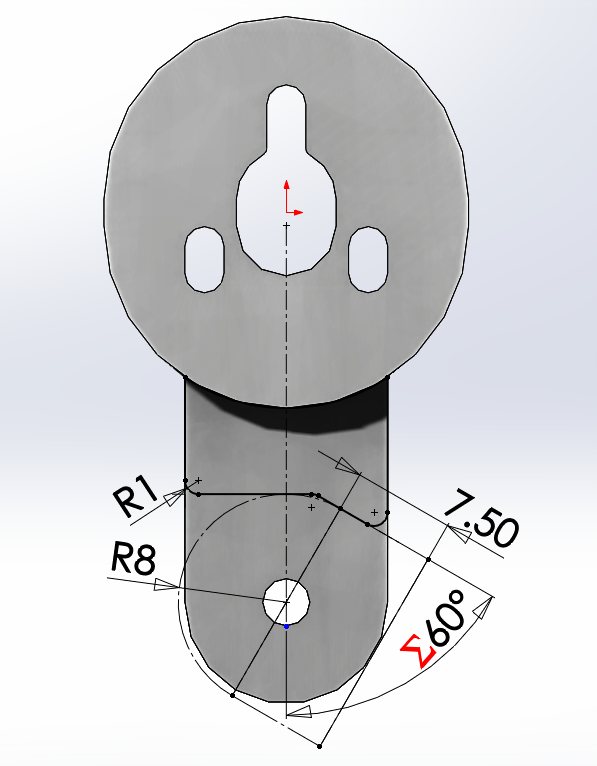
\includegraphics[width=\textwidth]{figures/joint_limits_hip.PNG}
        \caption{Joint limits of the hip}
        \label{fig:joint_limits_hip}
    \end{subfigure}
    \begin{subfigure}[b]{0.49\textwidth}
        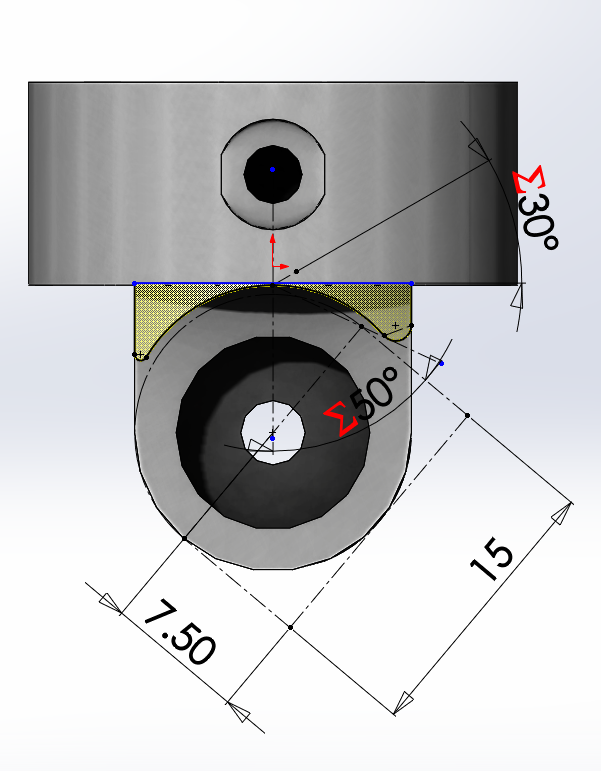
\includegraphics[width=\textwidth]{figures/joint_limits_ankle_upper.PNG}
        \caption{Joint limits of the ankle}
        \label{fig:joint_limits_ankle_upper}
    \end{subfigure}
\end{figure}    

\begin{figure}[ht!]
    \ContinuedFloat % continue from previous page
    \begin{subfigure}[b]{0.49\textwidth}
        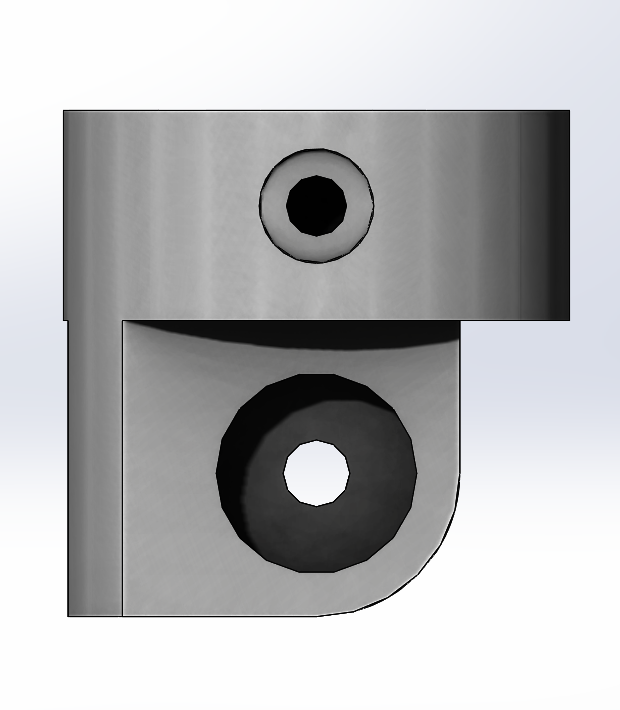
\includegraphics[width=\textwidth]{figures/joint_limits_knee_upper.PNG}
        \caption{Joint limits of the knee: Upper link}
        \label{fig:joint_limits_knee_upper}
    \end{subfigure}
    \begin{subfigure}[b]{0.49\textwidth}
        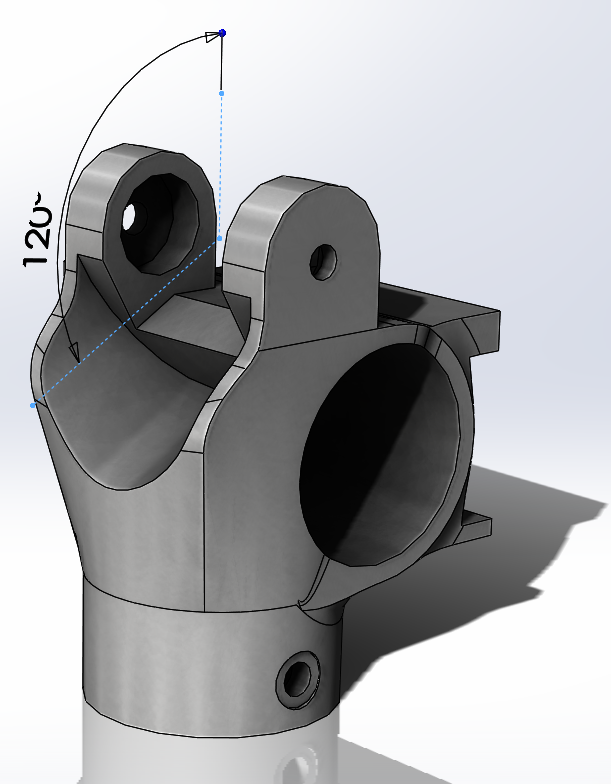
\includegraphics[width=\textwidth]{figures/joint_limits_knee_lower.PNG}
        \caption{Joint limits of the knee: Lower link}
        \label{fig:joint_limits_knee_lower}
    \end{subfigure}
\end{figure}    

% subsection mechanical_limits (end)